\documentclass[12pt, onecolumn]{article}

\usepackage{mystyle}
\graphicspath{{./figs/}}

% Document
\begin{document}

\title{\bf{Transferring Entanglement Between Different Dimensions}} 
\date{Submitted: \today{}}
\author{
    Timothy Forrer\\
    Level 4 Project, MSci Natural Sciences\\
    Supervisor: Dr V. Kendon\\
    Department of Physics, Durham University}

\maketitle

\begin{abstract}              
 
    Entangled qudit states, which share higher dimensional entanglement, enable quantum computers to unlock greater advantages in the computations that they are able to perform.
    As such, the generation of these entangled states is a worthy problem to consider as quantum computing technology becomes more and more advanced.
    Many methods of generating Bell pair entangled qubits have been proposed and realised, but schemes for qudit pairs of arbitrary dimension are not as well-researched.
    A protocol utilising quantum walk dynamics has been proposed to repeatedly transfer bipartite entanglement from Bell pairs to be accumulated in qudit pairs.
    Analysis of this protocol shows that this transfer is not optimal when using true quantum walk dynamics.
    Due to its non-unitary nature, it is also not easily reversed to retrieve entanglement from higher dimensional entangled states. Post-selection is also needed, where states are sometimes discarded and the entire protocol has to be repeated.
    An adapted version of the protocol, given as a circuit of gates conforming to ancilla-based quantum computing constraints rather than quantum walk ones, is proposed as an alternative which is able to achieve optimal entanglement transfer.
    It allows for entanglement to be transferred freely between qubit and qudit pairs as it is fully unitary and hence reversible.
    Furthermore, it is shown that with the addition of a single gate, the circuit can be used to turn qudits into a form of quantum random access memory.
    
\end{abstract}

\newpage

\tableofcontents

\newpage

\section{Introduction}
\label{section:intro}
Quantum walks are powerful tools in the landscape of quantum computing. 
Much like their classical analogues, they exhibit many properties that are desirable for computations and are an extremely useful building block for many algorithms designed for quantum computers \cite{shenvi2003}. 
However, they also have some very significant divergences from classical random walks, including a quadratic speed up in their spreading, and quantum correlations that have no classical comparison. 
Their power is such that it has been shown that quantum walks can simulate any quantum computation and therefore are a model for universal quantum computing \cite{Childs_2009}.
There is also evidence of robust performance even when the quantum computer is not perfectly isolated from its environment, leading to situations where decoherences due to interactions with the environment is beneficial for a given computation \cite{KENDON_2007}. 
It is possible to divide quantum walks into two categories, discrete time and continuous time. 
The latter have been shown to solve a wide range of problems in a number of different settings. 
However, the focus of this report will be on entangled state generation and transfer which neccessitates the need for more than one Hilbert subspace in our system, a setting which lends itself much more readily to discrete time quantum walks.\newline

Quantum walks have been shown to have great versitility in the generation and transfer of entanglement, quantum correlations which have no classical analogue, within a quantum system. 
Entanglement is a key resource for many quantum computing protocols \cite{qkd}\cite{Superdense}\cite{qteleport}, and is the source of the quadratic speedup evident in so many quantum algorithms that best their classical counterparts.\newline

In this report we will first review discrete quantum walks on different graphs in section 2. 
Section 3 will then discuss using discrete quantum walks in order to transfer entanglement between subspaces within a quantum walk system. 
Finally, a short summary is presented in section 4.\newline

As mentioned above, discrete time quantum walks are much more suited for the purposes of this report, therefore future references to quantum walks will be assumed to be the discrete variant unless stated otherwise. 
We will also use Q.W. to denote (discrete) quantum walk. 
The mathematical notation used in this report follows standard conventions, however it's worth making clear the equivalency between $\ket{u_1}\ket{u_2} \equiv \ket{u_1} \otimes \ket{u_2}$, where both forms will be used interchangeably.

\section{Background}
\label{section:background}
\subsection{Quantum Computation}
\subsubsection{Qubits}
\label{subsubsection:qubits}
A qubits can be described by a state belonging to a Hilbert space $\mathcal{H}$ of dimension two.
A common basis for $\mathcal{H}$ is \emph{computational basis}, labelled by $\ket{0}$ and $\ket{1}$.
Naturally we can also use other bases for describing our qubit state. A common alternative is the basis $\{\ket{+}, \ket{-}\}$.
This basis is best known as the \emph{Hadamard basis}, as $\ket{+}$ and $\ket{-}$ are equal to $H\ket{0}$ and $H\ket{1}$, where $H$ is the Hadamard transform given by
\begin{align}
    \ket{+} &= H\ket{0} = \frac{1}{\sqrt2} \left(\ket{0} + \ket{1}\right)\\
    \ket{-} &= H\ket{1} = \frac{1}{\sqrt2} \left(\ket{0} - \ket{1}\right).
\end{align}
Qubits can also be written out in vector form, and the most common choice for this is to assign the computational basis states as
\begin{align}
    \ket{0} = 
    \begin{pmatrix}
        1 \\
        0
    \end{pmatrix}, \;
    \ket{1} = 
    \begin{pmatrix}
        0 \\
        1
    \end{pmatrix}.
\end{align}
Therefore the Hadamard transform and associated basis states are given by
\begin{equation}
    \begin{gathered}
        H = \frac{1}{\sqrt{2}}
        \begin{pmatrix}
            1 & 1\\
            1 & -1
        \end{pmatrix}\\
        \ket{+} = \frac{1}{\sqrt{2}}
        \begin{pmatrix}
            1 \\
            1
        \end{pmatrix}, \;
        \ket{-} = \frac{1}{\sqrt{2}}
        \begin{pmatrix}
            1 \\
            -1
        \end{pmatrix}.
    \end{gathered}
\end{equation}

\subsubsection{Qudits}
\label{subsubsection:qudits}
In quantum computing, or indeed classical computing, there is no physical constraint that necessitates the use of two level qubits or bits.
In classical computing, the bit can be generalised to a unit that takes on one of $d$ states, known as the \emph{dit}.
Similarly, the quantum dit is the \emph{qudit}, which can be in superposition of up to $d$ states.
Many aspects of quantum computing specific to qubits generalise nicely to qudits.
The computational basis is now extended from $\{\ket{0}, \ket{1}\}$ to $\{\ket{i}\}_{i=0}^{d-1}$.
To distinguish kets representing belonging to Hilbert spaces of different dimension, the notation $\ket{\cdot}_d$ will be used to denote a state belonging to a Hilbert space $\mathcal{H}_d$ where denotes a Hilbert space of dimension $d$.
For compactness, operators will not have their dimension explicitly labelled, since they belong to the same Hilbert space as the state they are acting on.
Similar to qubits, there are many different bases that can be used to describe our qudit states.
The $d$ dimensional analogue to the Hadamard transform is the \emph{quantum Fourier transform} is given by
\begin{equation}
    F\ket{x}_d = \frac{1}{2^{\frac{d}{2}}} \sum_{y=0}^{d-1} \omega^{xy}\ket{y}_d,
\end{equation}
where $\omega = e^{i\frac{2\pi}{d}}$, i.e. it is the $d^{th}$ root of unity.
Therefore the Fourier basis can be generalised to the set of states  $\{\ket{+_i}\}_{i=0}^{d-1}$, where
\begin{equation}
    \ket{+_i}_d = F\ket{i}_d.
\end{equation}
Note that in the case $d=2$, $F = H$, hence the Hadamard transform is actually a quantum Fourier transform.\newline

Again, qudits can also be written as vectors, with the computational basis states again assigned as
\begin{equation}
    \ket{0} = 
    \begin{pmatrix}
        1 \\
        0 \\
        \vdots\\
        0
    \end{pmatrix}, \;
    \ket{1} = 
    \begin{pmatrix}
        0 \\
        1 \\
        \vdots \\
        0
    \end{pmatrix}, \dots, \;
    \ket{d - 1} =
    \begin{pmatrix}
        0 \\
        0 \\
        \vdots \\
        1
    \end{pmatrix}.
\end{equation}
The Fourier transform can also be given as the matrix
\begin{equation}
    F = \begin{pmatrix}
        1 & 1 & \cdots & 1\\
        1 & \omega & \cdots & \omega^{d-1}\\
        \vdots & \vdots & \ddots & \vdots\\
        1 & \omega^{d-1} & \cdots & \omega^{{(d-1)}^2}
    \end{pmatrix},
\end{equation}
and the associated Fourier basis states are found by applying the matrix representation of $F$ to the computational basis state vectors.

\subsubsection{Collections of Qudits}
\label{subsubsection:collections_qbits}
Qudits considered in isolation are not overly useful for quantum computations and in general a collection of qudits is needed for a given algorithm.
The Hilbert space of a collection of $n$ qudits, which are not neccessarily all of the same dimension, is found by taking the tensor product, $\otimes$, of the Hilbert spaces of each of the individual qudits
\begin{equation}
    \mathcal{H} = \mathcal{H}_{d_0} \otimes \mathcal{H}_{d_1} \otimes \dots \otimes \mathcal{H}_{d_{n-1}}.
\end{equation}
The computational basis state for the combined Hilbert space is found by taking all possible tensor product combinations of the basis states for each constituent Hilbert space.
The state 
\begin{equation}
    \ket{0}_{d_0}\otimes\ket{0}_{d_1}\otimes\dots\otimes\ket{0}_{d_{n-1}}
\end{equation}
is an example of such a basis state.
Notationally, this state can be further simplified by the omission of the tensor product symbol,
\begin{equation}
    \ket{0}_{d_0}\ket{0}_{d_1}\dots\ket{0}_{d_{n-1}}.
\end{equation}
If the kets are of the same dimension then this can be further compactified by contracting them,
\begin{align}
    \ket{0}_{d}\ket{0}_{d}\dots\ket{0}_{d} = \ket{00\dots0}_d.
\end{align}
Since tensor products distribute over sums, when combining states in superposition they must also be distributed over.
For example with two qudits,
\begin{align}
    (\ket{0}_d + \ket{1}_d)\otimes\ket{2}_d &= (\ket{0}_d + \ket{1})_d\ket{2}_d\\
    &= \ket{02}_d + \ket{12}_d
\end{align}
Recall also from the properties of the tensor product that it is not commutative, therefore care must be taken in ensuring that the order of qudits is preserved throughout,
\begin{equation}
    \ket{01}_2 \neq \ket{10}_2.
\end{equation}
In this report all three notational methods are used, with clarity given due preference over compactness.
The subscripts are often dropped when the meaning is clear.

\subsubsection{Operators}
\label{subsubsection:operators}
There are a wide variety of other operators beyond those introduced above that equate to a change of bases.
One of the most common is the (Pauli) $X$, or NOT, operator.
As the second name implies, in the qubit setting acts in the same way as the classical NOT operator,
\begin{align}
    \ket{0} &\mapsto \ket{1}\\
    \ket{1} &\mapsto \ket{0}.
\end{align}
More generally in the qudit setting,
\begin{equation}
    X\ket{i}_d = \ket{i + 1 \text{ mod } d}_d.
\end{equation}
However, there are other gates that do not have a classical analogue such as the  the (Pauli) $Z$ gate.
In the qubit setting acts $Z$ as the identity on $\ket{0}$ and applies a relative phase to $\ket{1} \mapsto -\ket{1}$.
Again this can be generalised to the qudit setting
\begin{equation}
    Z\ket{i}_d = \omega^i\ket{i}_d,
\end{equation}
where $\omega$ is again the $d^{th}$ root of unity.
Both of these operators are sometimes referred to as Pauli operators as their matrix representations in the computational basis are given by the Pauli matrices $\sigma_x$ and $\sigma_z$.
There is also the $Y$ operator corresponding to the Pauli $\sigma_y$ matrix but this is often omitted from consideration as
\begin{equation}
    ZX = iY.
\end{equation}
Hence when designing a set of operators for a quantum computer, there is no theoretical need for $Y$ as it already exists up to a global phase, which is essentially irrelevant.
The final operation to be introduced in the section is the $\C{U}$, or controlled-$U$ operator, where $U$ is any unitary operation.
This operator is distinct from the others previously introduced in that it acts on two qudits rather than just one, although it only directly alters the state of one of the two qudits.
In the qubit setting, one qubit is designated as the control qubit and the other the target.
If the control qubit is in the state $\ket{0}$, then nothing happens to the target qubit.
If the control qubit is in the state $\ket{1}$, then the operator $U$ is applied to the target qubit.
Written mathematically, where the left hand qubit is the control, the right hand qubit is the target in some arbitrary qubit state $\ket{\psi}$,
\begin{align}
    \C{U}\left(\ket{0}\otimes\ket{\psi}\right) &= \ket{0}\otimes\ket{\psi}
    \label{eq:controlled_0}\\
    \C{U}\left(\ket{1}\otimes\ket{\psi}\right) &= \ket{1}\otimes U\ket{\psi}.
    \label{eq:controlled_1}
\end{align}
To extend this to the qudit setting, first note that \crefrange{eq:controlled_0}{eq:controlled_1} can be compactly written as
\begin{equation}
    \C{U}\left(\ket{x}\otimes\ket{\psi}\right) = \ket{x}\otimes U^x\ket{\psi}.
    \label{eq:controlled_x}
\end{equation}
This equation now is well-defined for qudits, where instead of just taking values $0$ or $1$, $x$ can now take values from $\{0, 1, \dots, d-1\}$.
Note that this definition applies also when the dimensions of the control and target are not equal, provided that the action of $U$ on the target is well-defined
\begin{equation}
    \C{U}\left(\ket{x}_d\otimes\ket{\psi}_{d'}\right) = \ket{x}_d\otimes U^x\ket{\psi}_{d'}.
\end{equation}
In this report, unless otherwise stated, it is assumed that control qudits are always on the left and target qubits on the right.\newline

It is sometimes neccessary to have operators that act on single qudits in a collection of $n$ qudits.
These can be expressed by taking the tensor product with the identity acting on the other qudits in the collection.
For example, the operator that acts with an $X$ on the qudit of index 1 in the state $\ket{\psi_0}\otimes\ket{\psi_1}\otimes\ket{\psi_2}$ is given by
\begin{equation}
    I\otimes X\otimes I.
\end{equation}

\subsubsection{Circuits and Gates}
\label{subsubsection:circuits_and_gates}
When describing a circuit that implements a series of operators on our qudits, it is often much clearer and simpler to use a circuit diagram.
Straight lines in the circuits represent qubits/qudits.
Operations on qudits are represented by gates placed on the straight lines corresponding to the qudits we wish to act on.
A table of gates relevant for this report is given in table \ref{table:gates}.
\begin{table}
    \begin{center}
        \begin{tabular}{c | c}
            Operator & Gate\\
            \hline
            (Pauli) X & \begin{tikzcd} \qw & \gate{X} & \qw \end{tikzcd}\\
            (Pauli) Z & \begin{tikzcd} \qw & \gate{Z} & \qw \end{tikzcd}\\
            Hadamard & \begin{tikzcd} \qw & \gate{H} & \qw \end{tikzcd}\\
            QFT & \begin{tikzcd} \qw & \gate{F} & \qw \end{tikzcd}\\
        \end{tabular}
        \caption{Table of operators and their gate representations in quantum circuits.}
        \label{table:gates}
    \end{center}
\end{table}

When reading a circuit, time flows from left to right and a gate must finish its operation on a qudit before the next gate on the same qudit is enacted. Figure \ref{fig:sample_circuit} is an example of a two qubit circuit implementing the following series of operations
\begin{equation}
    \C{X}(Z\otimes I)(X\otimes I)\left(\ket{0}_2\otimes\ket{\psi}_2\right).
    \label{eqn:sample_operations}
\end{equation}

\begin{figure}
    \begin{center}
        \begin{tikzpicture}
            \node[scale=1.0] {
                \begin{quantikz}
                    \lstick{$\ket{0}_2$} & \gate{X} & \gate{Z} & \ctrl{1} & \qw\\
                    \lstick{$\ket{\psi}_2$} & \qw & \qw & \targ{} & \qw
                \end{quantikz}
            };
        \end{tikzpicture}
    \caption{An example of a circuit schematic representing the expression given in equation \ref{eqn:sample_operations}.}
    \label{fig:sample_circuit}
    \end{center}
\end{figure}
\label{subsection:qc_primer}
\subsection{Entanglement}
Entanglement is a property of quantum systems that is the source of many of the remarkable results displayed by quantum algorithms.
Essentially it is the presence of correlations in a quantum system that is stronger than possible classically.
Although entanglement can exist between multipartite systems, such as in the case of GHZ states or W states, in this report only bipartite entanglement will be discussed.
Therefore, all references to entanglement are specifically referring to bipartite entanglement.
Generalising entanglement to higher dimensions in the bipartite setting is done by having entanglement between qudits as opposed to qubits.
There is no requirement for the dimensions of the entangled qudits to be matching.
For example,
\begin{equation}
    \ket{\psi} = \frac{1}{\sqrt{2}}\left(\ket{0}_2\otimes\ket{0}_3 + \ket{1}_2\otimes\ket{1}_3\right),
\end{equation}
is a entangled state between a qubit and a qutrit ($d=3$).

\subsubsection{Measuring entanglement}
\label{subsubsection:measure_entanglement}
In order to analyse the efficiency of an entanglement transfer protocol, it is useful to have a method of measuring entanglement, of which numerous methods have been proposed and are used.
For a full mathematical discussion on entanglement quantification, see \cite{Plenio_2007}.
In this report, the measure of entanglement used is the \emph{logarithmic negativity}, first presented by Vidal \cite{Vidal_2002}.
\begin{definition}[Logarithmic Negativity]
    \label{definition:log_neg}
    Let $\rho$ be a density matrix describing a bipartite quantum system $\mathcal{H} = \mathcal{H}_A \otimes \mathcal{H}_B$.
    The logarithmic negativity, $E_\mathcal{N}(\rho)$, of $\rho$ is defined as
    \begin{equation}
        E_\mathcal{N}(\rho) = \log_2\left\Vert \rho^{\Gamma_A}\right\Vert_1.
    \end{equation}
    where $\rho^{\Gamma_A}$ denotes the partial transpose of $\rho$ with respect to the subsystem $\mathcal{H}_A$ and $\Vert X\Vert_1 = Tr(\sqrt{X^\dagger X})$ denotes the trace norm of $X$.
\end{definition}
The logarithmic negativity is also referred to as the log negativity.
It is an appropriate choice for the purpose of this report as it is an entanglement measure that is computable for mixed as well as pure states, and satisfies (strong) additivity
\begin{equation}
    E_\mathcal{N}(\rho \otimes \sigma) = E_\mathcal{N}(\rho) + E_\mathcal{N}(\rho).
\end{equation}
A proof for this is given in \cite{Vidal_2002}.\newline
This usefulness of this can be demonstrated with the use of the following claim.
\begin{claim}
    \label{claim:maximally_entangled_states}
    A maximally entangled state in $d\times d$ dimensions has a log negativity of $\log_2d$.
\end{claim}
\begin{proof}
    First, note that for a Hilbert space of dimension $d\times d$, the state
    \begin{equation}
        \ket{\psi} = \frac{1}{\sqrt{d}}\sum_{j=0}^{j=d-1}\ket{j}\otimes\ket{j}\in \mathcal{H}_A \otimes \mathcal{H}_B
    \end{equation}
    is maximally entangled, since its reduced density matrix in either subspace is maximally mixed.
    So to quantify the entanglement of any maximally entangled state it is sufficient to calculate the log negativity of the density matrix, $\rho$ associated with $\ket{\psi}$.
    Since $\ket{\psi}$ is a pure state
    \begin{align}
        \rho &= \ket{\psi}\bra{\psi}\\
        &=\frac{1}{d} \sum_{j,k}\ket{j}\bra{k}\otimes\ket{j}\bra{k}
    \end{align}
    To calculate $E_{\mathcal{N}}(\rho)$ we need the partial transpose on one of the subspaces, the choice of which is irrelevant since they are both equally entangled with one another.
    So choose to find the partial transpose in $\mathcal{H}_A$.
    \begin{align}
        \rho^{\Gamma_A} =\frac{1}{d} \sum_{j,k}\ket{k}\bra{j}\otimes\ket{j}\bra{k}
    \end{align}
    From this we wish to calculate the trace norm $\Vert X\Vert_1 = \Tr\left(\sqrt{XX^{\dagger}}\right)$.
    \begin{align}
        \rho^{\Gamma_A}\left(\rho^{\Gamma_A}\right)^{\dagger} &= \frac{1}{d^2} \sum_{j,k}\ket{k}\bra{k}\otimes\ket{j}\bra{j}\\
        &=\frac{1}{d^2}I_d\otimes I_d\\
        &=\frac{1}{d^2}I_{d^2}\\
        \implies \Vert\rho^{\Gamma_A}\Vert_1 &= \frac{1}{d}\Tr{\left(I_{d^2}\right)}\\
        &= \frac{1}{d}\cdot d^2\\
        &= d
    \end{align}
    Therefore, this gives
    \begin{align}
        E_{\mathcal{N}} &= \log_2\left\Vert \rho^{\Gamma_A}\right\Vert\\
        &= \log_2d.
    \end{align}
\end{proof}
This combined with the strong additivity condition is what makes the choice of log negativity an apt one.
In comparing how efficient the transfer of entanglement from the Bell pairs to a qudit pair, the log negativity allows for direct comparison of the entanglement transferred into the two qudit system, and the entanglement of the resultant state of the qudit pair.
If the entanglement in $n$ Bell states is transferred, then the final state of the qudit pair has log negativity $n$ in the case of optimal transfer.
\label{subsection:entangle}
\subsection{Random Walks}
\subsubsection{Classical Random Walk}
Before discussing quantum random walks, I will first motivate their design using the example of a classical random walk on a discrete number line.
In the classical random walk, a walker (often described as being somewhat inebriated) is constrained to moving up and down a discrete number line, starting their walk at the origin.
To determine whether to take a step to the left (-1) or the right (+1), the walkers flips an unbiased coin, moving to the right if the coin lands on heads and to the left if the coin lands on tails. 
The process is can be repeated over and over until a desired stopping point is reached, after a given number of coin flips, or until the walker has reached a specific destination, such as their house in the case of the inebriated walker.
The walk can also continue on forever and in this limit, the walker will reach every point on the number line.
The probability distribution describing the probability of the walker being in any given position away from the origin is given by a binomial distribution, shown in orange in Figure \ref{fig:discVSclass} for 100 coin flips. 

\subsubsection{Quantum Random Walk}
With the classical random walk model in mind, we are now in a position to "quantise" it into the \emph{quantum random walk}.
In our walker system, we can divide the overall Hilbert space of the QW, $\mathcal{H}$, into two subspaces, the coin subspace $\mathcal{H}_C$ and the position subspace of the walker $\mathcal{H}_W$. 
\begin{equation}
    \mathcal{H} = \mathcal{H}_C \otimes \mathcal{H}_W.
\end{equation}
To aid distinguishability between coin states and position states, we write that
\begin{align}
    \langle\mathcal{H}_C\rangle &= \{\ket{\uparrow}, \ket{\downarrow}\}\\
    \langle\mathcal{H}_W\rangle &= \{\ket{k} | k\in\mathbb{Z}\},
\end{align}
where $\langle U \rangle$ denotes a set of vectors which span $U$. 
Therefore, the states $\ket{\uparrow}, \ket{\downarrow}$ take the place of heads and tails on our quantum "coin". 
Note in particular that there is no constraint placed on the dimensionality of $\mathcal{H}_W$, and therefore the walker can be taken to be a qudit, whereas $\dim{\mathcal{H}_C} = 2$ and the coin is taken to be a qubit.
Having defined the Hilbert space within which the walk will be conducted, we can now define operators within our space that will dictate how the QW will proceed. We first define the "coin flip" operator $C\in \mathcal{H}_C$. 
There is a continuum of choices for $C$, details of which can be found here \cite{Tregenna2003}. 
For walks on a line, if we restrict ourselves to choosing an unbiased coin with real coefficients the Hadamard coin is the only choice of coin available.
This takes on the same form as the Hadamard transform defined in Section \ref{subsection:qc_primer},
\begin{align}
    C &= \frac{1}{\sqrt{2}}\Big[
    \ket{\uparrow}\bra{\uparrow} +
    \ket{\uparrow}\bra{\downarrow} +
    \ket{\downarrow}\bra{\uparrow} -
    \ket{\downarrow}\bra{\downarrow}\Big]\\
    &= \frac{1}{\sqrt{2}}\Big[(\ket{\uparrow} + \ket{\downarrow})\bra{\uparrow} +
    (\ket{\uparrow} - \ket{\downarrow})\bra{\downarrow}\Big]
    \label{equation:hadamard_coin}
\end{align}
where $\ket{0} \rightarrow \ket{\uparrow}$ and $\ket{1} \rightarrow \ket{\downarrow}$.
Equation \ref{equation:hadamard_coin} makes obvious the action of $C$; if the coin state is $\ket{\uparrow}$ then it becomes an equal superposition of $\ket{\uparrow} + \ket{\downarrow}$, if the coin state is in $\ket{\downarrow}$ then we get an equal superposition of $\ket{\uparrow} - \ket{\downarrow}$. 
These two equal superpositions are often denoted as $\ket{+}$ and $\ket{-}$ respectively.\newline
We then define our shift operator $S \in \mathcal{H}$ which allows the position of our walker to change, dependent on the state of the coin.
\begin{equation}
    S = \sum_k \ket{\uparrow}\bra{\uparrow} \otimes \ket{k + 1}\bra{k} + \ket{\downarrow}\bra{\downarrow} \otimes \ket{k - 1}\bra{k}.
\end{equation}
Again, this representation of $S$ makes manifest its effect on our walker. 
If the coin is in the $\ket{\uparrow}$, then we take a step in the +1 direction, if in the $\ket{\downarrow}$ then we take a step in the -1 direction. 
The probability distribution of such a walk is plotted in Fig \ref{fig:discVSclass}, where the initial coin state is $\ket{\downarrow}$, and is compared to a classical random walk.\newline

\begin{figure}
    \centering
    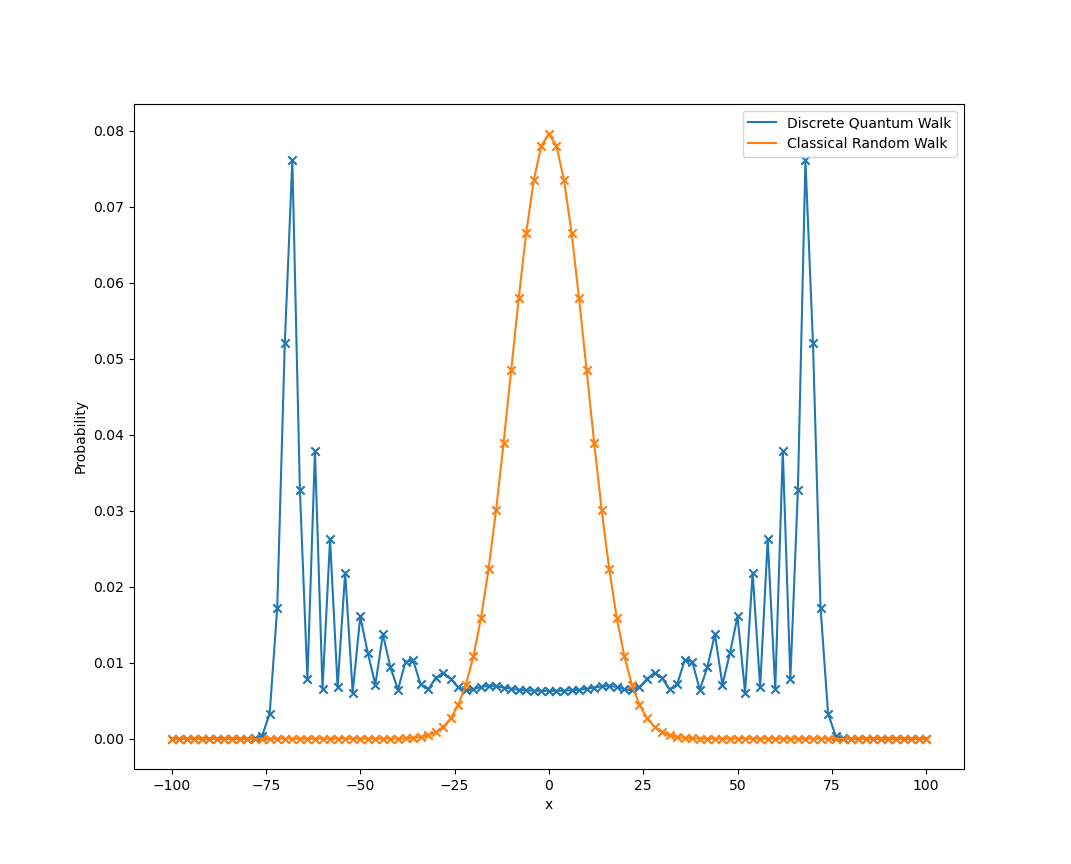
\includegraphics[scale=0.75]{Discrete vs Classical Walk.png}
    \caption{The probability distributions of a classical and quantum walk on a line, both originating at the origin. The quantum walk coin is initially in the $\frac{1}{\sqrt{2}}\left(\ket{\uparrow} + i\ket{\downarrow}\right)$ state. Odd points have been omitted as they all have zero probability.}
    \label{fig:discVSclass}
\end{figure}

Whilst the above choice of $S$ is the most common on the number line, it is also possible to define an alternative choice of shift operator,
\begin{equation}
    \tilde{S} = \sum_k \ket{\uparrow}\bra{\uparrow} \otimes \ket{k}\bra{k} + \ket{\downarrow}\bra{\downarrow} \otimes \ket{k + 1}\bra{k}.
\end{equation}
Th subtle difference between $\tilde{S}$ and $S$ is that $\tilde{S}$ can only move in the $+1$ direction of the number line and has no "left moving" part, so to speak. 
This means that $\tilde{S}$ is restricted to the non-negative integers and unlike $S$, can occupy all $\ket{x}$ for $0\leq x\leq T$, where $T$ is the number of time steps in our QW.

\FloatBarrier
\label{subsection:qw}
\subsection{Ancilla-Based Quantum Computing}
Quantum walks is but one of many universal quantum computing models.
Another model is known as \emph{ancilla-based quantum computing}, which, in particular, aims to resolve two conflicting demands when building quantum computers:
We wish for our qubits to be well isolated to prevent decoherence, yet also want them to interact with each other to perform our quantum computations.
However, a qubit cannot distinguish between unwanted and wanted interactions, resulting in the need for a balancing act that adequetely addresses these two issues.

Ancilla-based quantum computing aims to resolve this conflict by using additional qubits, known as ancilla qubits, which mediate interactions between the main register qubits. 
Using this model, it is possible to implement two complementary registers of qubits.
The main register can be designed to be strongly isolated from interactions, bar a select few natural interactions with the ancilla registry, whose qubits can be easily manipulated but decohere much faster. Quantum computations can be performed by \emph{delocalising} quantum information from the main register across both the register and the ancilla. After performing a computation on the ancilla qubit, the quantum information is then \emph{relocalised} back into the main register.
The ancilla can be reset to the initial state and used again for other computations.
A simple example of a circuit designed for ancilla-based quantum computing is shown in Figure \ref{simple aqc}. 

\begin{figure}[h]
    \begin{center}
        \begin{tikzpicture}
            \node[scale=1.0] {
                \begin{quantikz}
                    \lstick{$\ket{\psi}$} & \ctrl{1} & \qw &\ctrl{1} & \qw\\
                    \lstick{$\ket{0}$} & \targ{} & \gate{Z} & \targ{} & \qw
                \end{quantikz}
                $\equiv$
                \begin{quantikz}
                    \lstick{$\ket{\psi}$} & \gate{Z} & \qw
                \end{quantikz}
            };
        \end{tikzpicture}
    \caption{Two circuits that implement a $Z$ gate acting on an arbitrary qubit $\ket{\psi}$.}
    \label{simple aqc}
    \end{center}
\end{figure}
The circuit on the left hand side of Figure \ref{simple aqc} does not directly implement any unitary transformations on an arbitrary qubit state $\ket{\psi} = \alpha \ket{0} + \beta \ket{1}$, but instead indirectly acts on $\ket{\psi}$ via the ancilla qubit, to which the quantum information of $\ket{\psi}$ is shared to via a CNOT gate. Acting a $Z$ gate on the ancilla and relocalising the quantum information with another CNOT gate "passes on" the effects of the $Z$ gate.
This model of quantum computing does not have to be reserved to qubit computing alone and applies to qudits and even quantum continous variables (QCVs).
However, here the focus will be on utilising it with qubits and qudits.
In fact there is no prerequisite to only using qudits of similar dimension, and defining quantum operators designed for mismatched dimensions is relatively straightforward to do.
First examine the the case of the controlled NOT gate.
In Section \ref{subsection:qc_primer} it was shown that the $\C{X}$ gate acts an $X$ gate on the target qubit if the control qubit is in the state $\ket{1}$. This can be summarised as follows
\begin{equation}
    \C{X}\left(\ket{i}_2\otimes\ket{j}_2\right) = \ket{i}_2 \otimes X^i\ket{y}_2.
\end{equation}
Expressed in this way there is quite a natural extension of the $\C{X}$ gate in the case that the control and target are both qudits of arbitrary dimension,
\begin{equation}
    \C{X}\left(\ket{i}_d\otimes\ket{j}_{d'}\right) = \ket{i}_d \otimes X^i\ket{y}_{d'},
\end{equation}
recalling that the general $X$ gate in $d'$ dimensions increments the basis states by 1, mod $d'$.
Indeed any $\C{U}$ gate can be expressed in this manner
\begin{equation}
    \C{U}\left(\ket{i}_d\otimes\ket{j}_{d'}\right) = \ket{i}_d \otimes U^i\ket{y}_{d'},
\end{equation}
provided that $U$ has been well-defined in $d'$ dimensions.

Later in this report I will highlight how this particular model of quantum computing is well suited for the protocol outlined in \cite{giordani2020}, which will be discussed in detail in the following section.

\label{subsection:aqc}

\section{Entanglement Transfer using Quantum Walks}
\label{section:qw_transfer}
Here the protocol presented in \cite{giordani2020} which utilises quantum walk dynamics in order to generate higher dimensional entanglement is summarised.

The imagined setup of this protocol is that there are two labs, $A$ and $B$, which have a shared source of entangled qubits but are otherwise spatially separated and cannot interact with one another.

In this section we use following notation:
\begin{itemize}
    \item $\ket{\psi}_J$ is a state belonging to the subspace $\mathcal{H}_J = \mathcal{H}^{(A)}_J \otimes \mathcal{H}^{(B)}_J, J\in\{C,W\}$.
    \item $\ket{\psi}^{(K)}$ is a state belonging to the subspace $\mathcal{H}^{(K)} = \mathcal{H}^{(K)}_C \otimes \mathcal{H}^{(K)}_W, K\in\{A,B\}$.
    \item  $\ket{\psi}^{(K)}_J$ is a state belonging to the subspace $\mathcal{H}^{(K)}_J$.
\end{itemize}

In this mathematical framework the overall Hilbert space is comprised of two quantum walk subspaces,
\begin{align}
    \mathcal{H} &= \mathcal{H}^{(A)} \otimes \mathcal{H}^{(B)}\\
                &= \mathcal{H}^{(A)}_C \otimes \mathcal{H}^{(A)}_W \otimes \mathcal{H}^{(B)}_C \otimes \mathcal{H}^{(B)}_W.
\end{align}
Although due to the difficulty in writing entangled states when the entangled spaces are not adjacent, states will be written with the following ordering
\begin{equation}
    \mathcal{H} = \mathcal{H}^{(A)}_W \otimes \mathcal{H}^{(B)}_W \otimes \mathcal{H}^{(A)}_C \otimes \mathcal{H}^{(B)}_C,
\end{equation} 
i.e. with the walker subspaces adjacent to each other and the coin subspaces adjacent to each other.

The basic premise of this protocol is this:
\begin{enumerate}
    \item Entangle the two coin spaces of the walkers $\mathcal{H}^{(K)}_C$. (Fig \ref{fig:preparation}.)
    \item Proceed with the quantum walk for some determined number of steps.
    \item Use a projective measurement $\mathcal{P}_\gamma = \ket{\gamma}\bra{\gamma}, \ket{\gamma}\in\mathcal{H}^{(A)}_C$ to then transfer the entanglement so that it solely exists in the subspace $\mathcal{H}^{(A)}_W \otimes \mathcal{H}^{(B)}_C \otimes \mathcal{H}^{(B)}_W$.
    \item In similar fashion, find a projection $\mathcal{P}_\delta = \ket{\delta}\bra{\delta}, \ket{\delta}\in\mathcal{H}^{(B)}_C$ to transfer the entanglement to exist between the two walker subspaces, $\mathcal{H}^{(i)}_W$, only.
    \item Accumulate entanglement in the walker subspaces by once more entangling the two coin spaces and repeating the protocol.
\end{enumerate}

\begin{figure}
    \centering
    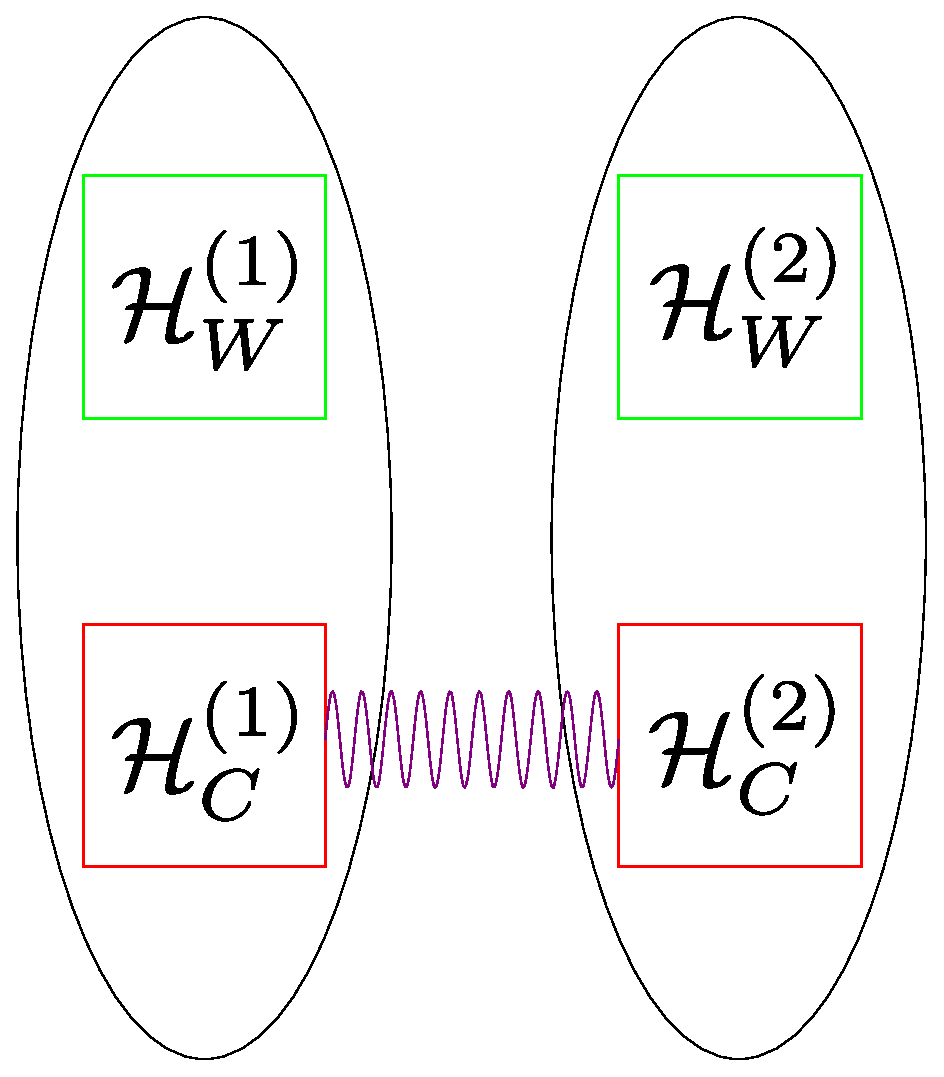
\includegraphics[scale = .25]{preparation}
    \caption{The initial prepared state has entanglement solely between the two coin subspaces. Figure is an edited version of FIG 3 from \cite{giordani2020}.}
    \label{fig:preparation}
\end{figure}
In this way, arbitrary amounts of higher dimensional entanglement can be generated.\newline
The ordering of steps 3 and 4 is not overly important since the full operators describing the projective measurements are given by
\begin{align}
    &\ket{\gamma}\bra{\gamma} \otimes I \otimes I \otimes I,\\
    &I \otimes \ket{\delta}\bra{\delta} \otimes I \otimes I
\end{align}
which clearly commute.
As is the case with many quantum walk based protocols, particular attention must be paid to the choice of coin used for the quantum walk, as it will have a large impact on the success of the protocol.
The shift operator used for the quantum walks is $\tilde{S}$, as outlined in section \ref{subsubsection:q_r_w}.
(Technically it is $\tilde{S}\otimes\tilde{S}$, one for each walk, but for the sake of brevity $\tilde{S}$ will be used.)

\subsection{Transfer using identity coin operator}
\label{subsection:qw_transfer}
To illustrate the basic principles of the protocol, consider the case where 
\begin{equation}
    C = \underbrace{I_2 \otimes I_2}_{\text{"Coin" operators}} \otimes I_d \otimes I_d = I.
\end{equation}
Note that this is not actual an instance of using quantum walk dynamics, since an identity coin equates to no coin at all.

\begin{enumerate}
    \item A state $\ket{\psi(0)}$ is prepared with the walkers at the origin and coin states entangled,
    \begin{equation}
        \ket{\psi(0)} = \ket{0}^{(A)}_W\ket{0}^{(B)}_W \otimes \underbrace{\frac{1}{\sqrt{2}}\Big [\ket{\uparrow}^{(A)}_C\ket{\uparrow}^{(B)}_C + \ket{\downarrow}^{(A)}_C\ket{\downarrow}^{(B)}_C \Big]}_{\text{Bell State}}.
    \end{equation}
    \item The "coin", $I$, is applied and followed by the shift operator $\tilde{S}$ to advance the quantum walk.
    Explicitly (dropping the indices and combining kets together) the walk evolves to the state
    \begin{equation}
        \ket{\psi(1)} = \tilde{S}I\ket{\psi} = \frac{1}{\sqrt{2}}\Big [\ket{0,0}\ket{\uparrow,\uparrow} + \ket{1,1}\ket{\downarrow,\downarrow}\Big].
    \end{equation}
    \item Using the operator $\mathcal{P}_{\gamma} = \ket{\gamma}\bra{\gamma}$ the part of $\ket{\psi(1)}$ residing in the $\mathcal{H}^{(A)}_C$ subspace is projected onto the state $\ket{\gamma}$.
    
    For this example, choose $\ket{\gamma} = \frac{1}{\sqrt{2}} \big [\ket{\uparrow} + \ket{\downarrow} \big]$ which then gives
    \begin{equation}
        \mathcal{P}_\gamma \ket{\psi(1)} = \frac{1}{2}\Big [\ket{0, 0}\ket{\gamma,\uparrow} + \ket{1, 1}\ket{\gamma, \downarrow}\Big ].
    \end{equation}
    \item Similarly, project the other coin onto $\ket{\delta}$ which in this instance is taken to be the same state $\ket{\delta} = \frac{1}{\sqrt{2}} \big [\ket{\uparrow} + \ket{\downarrow} \big]$,
    \begin{equation}
        \mathcal{P}_\delta \mathcal{P}_\gamma \ket{\psi(1)} = \frac{1}{2\sqrt{2}}\Big [\frac{1}{\sqrt{2}}\Big (\ket{0, 0} + \ket{1, 1}\Big )\ket{\gamma}\ket{\delta}\Big].
    \end{equation}
\end{enumerate}
Renormalising gives the final state
\begin{equation}
    \label{equation:qw_transfer_1_final}
    \underbrace{\frac{1}{\sqrt{2}}\Big [\ket{0, 0} + \ket{1, 1}\Big ]_W}_{\text{Bell State}}\otimes \ket{\gamma}^{(A)}_C \otimes \ket{\delta}^{(B)}_C,
\end{equation}
which has a Bell state in the $\mathcal{H}_W$ subspace, and the coin states are separable.
Therefore the entanglement that originally resided in the coin subspace has been transferred to the walker one.

\subsection{Accumulation}
\label{subsection:qw_accumulation}
The true motivation behind this protocol is the ability to accumulate the entanglement transferred from the lower dimensional coin subspace to the higher dimensional walker one.
This is done by repeating the entire process with some small changes.
Again $I$ is used as the coin.
\begin{enumerate}

    \item Starting with the final state obtained from the first iteration of the protocol (equation \ref{equation:qw_transfer_1_final}) the coin subspaces are re-entangled, obtaining a new initial state $\ket{\psi(0)}$,
    \begin{alignat}{3}
        \frac{1}{\sqrt{2}}
        \Big [\ket{0, 0} + \ket{1, 1}\Big ]_W\otimes \ket{\gamma}^{(A)}_C &\otimes \ket{\delta}^{(B)}_C\\
        \overset{\text{Entangle coins}}{\longrightarrow}
        \frac{1}{2}\Big [\ket{0, 0} + \ket{1, 1}\Big ]_W &\otimes
        \Big [\ket{\uparrow, \uparrow} + \ket{\downarrow, \downarrow}\Big ]_C& \\
        & &:=\ket{\psi(0)}.
    \end{alignat}
    \item Now take two steps instead of one in the walk.
    \begin{align}
        \ket{\psi(2)} &= (\tilde{S}I)^2\ket{\psi(0)}\\
        &= \frac{1}{2}\Big[\big (\ket{0,0}+\ket{1,1}\big )\ket{\uparrow,\uparrow} + \big (\ket{2,2} + \ket{3,3}\big )\ket{\downarrow,\downarrow}\Big ].
    \end{align}
    \itemrange{1} Using the same projection operators in the two coin subspaces, $\mathcal{P}_\gamma \in \mathcal{H}^{(A)}_C,  \mathcal{P}_\delta \in \mathcal{H}^{(B)}_C$, and renormalising gives the final state
    \begin{equation}
        \frac{1}{2}\Big[\ket{0,0} + \ket{1,1} + \ket{2,2} + \ket{3,3}\Big ] \otimes \ket{\gamma}\otimes\ket{\delta}.
    \end{equation}
\end{enumerate}

Using claim \ref{claim:maximally_entangled_states}, the log negativity of
\begin{equation}
    \frac{1}{2}\Big[\ket{0,0} + \ket{1,1} + \ket{2,2} + \ket{3,3}\Big ]
\end{equation}
is 2, setting $d=4$ (since both of the qudits only have 4 states of non-zero amplitude they can be simulated by ququarts even if their true dimension is greater than 4).
Therefore, 2 units of log negativity have been transferred from the Bell states (each of log negativity 1) to the qudit pair and optimal transfer has been achieved.
The process can be repeated to accumulate arbitrarily large amounts of entanglement into our walker subspace.
The number of steps needed in the quantum walk for each iteration is as follows.
\begin{claim}
\label{claim:min_steps}
The $n^{th}$ iteration (counting from 1) of the protocol requires $2^{n-1}$ steps in the quantum walk.
\end{claim}
\begin{proof}
Each step in a quantum walk with shift operator $\tilde{S}$ increases the number of basis states with non-zero amplitude by 1, provided that the amplitude $\ket{\downarrow}$ coin basis state is non-zero.
Therefore the dimension of each walker can be taken to be $s + 1$, where $s$ is the total number of steps taken in the walk, since each walker space can be reduced to the subspace spanned by the $s+1$ non-zero amplitude basis states.
Using claim \ref{claim:maximally_entangled_states}, the upper bound on the log negativity of the combined walker states after the $n^{th}$ iteration of the walk is given by $\log_2(s+1)$.
This implies the following condition on the total number of steps
\begin{equation}
    \log_2(s+1) = n \implies s = 2^n -1.
\end{equation}
This is an equality rather than an inequality $\log_2(s+1) \geq n$, since the state of the walkers is to be maximally entangled.
This means that the combined walker Hilbert space must be reducible to one of dimension $(s+1) \times (s+1)$.
This is only possible when taking the minimum number of steps (if more steps are taken then there are more than $s+1$ basis states of non-zero amplitude).
Assuming that this has been satisfied for the $n-1^{th}$ iteration of the protocol gives a total step number prior to the $n^{th}$ iteration of the walk of $s' = 2^{n-1} -1$ .
Therefore, the minimum number of steps for the $n^{th}$ iteration is given by
\begin{align}
    s - s' &= 2^{n} - 1 - (2^{n-1} -1)\\
    &= 2^n - 2^{n-1}\\
    &= 2 \times 2^{n-1} - 2^{n-1}\\
    &= 2^{n-1}.
\end{align}
\end{proof}

\subsection{Retrieval}
\label{subsection:qw_retrieval}
Although accumulating the entanglement in higher dimensions is of significant use, it is also possible to imagine that retrieving the entanglement back into the qubits would also be of use.
For example, consider the case where the method of generating entangled qubits is not deterministic but an algorithm requiring large numbers of Bell states is to be executed.
If the accumulation of entanglement can be reversed to get Bell pairs back, then the entangled Bell pairs can be stored in the qudits when they are successfully generated and then retrieved all at once to ensure the algorithm can be performed.
In principle, it is possible to use a similar quantum walk setup where the entangled qudits are the coins and the qubits are the walkers to get entanglement back out.
However due to the non-unitary nature of the protocol (the projective measurements are irreversible), this setup is not simple to design.

\subsection{Results}
\label{subsection:results}
Despite its simple construction, the state of a quantum walk becomes extremely complex after even just a few steps in most cases.
This is doubly true for two quantum walks running in conjunction.
Hence to analyse the protocol in settings that are not as trivial as the identity coin example, numerical simulations were run using Python and some associated packages \cite{numpy, scipy}.
Figure \ref{fig:2ebittransfer} shows that the protocol, when using a Hadamard coin, can generate a state with log negativity up to approximately 1.585 when the protocol is done twice, assuming both quantum coins are projected onto the same state $\ket{\gamma} = \cos{\theta}\ket{0} + e^{i\phi}\sin{\theta}\ket{1}$.
*****Simulations using different projective operators $\mathcal{P}_\gamma, \mathcal{P}_\delta$ show 1.585 is still the maximum possible.********
Hence a maximally entangled state cannot be generated with the Hadamard coin.
\begin{figure}
    \centering
    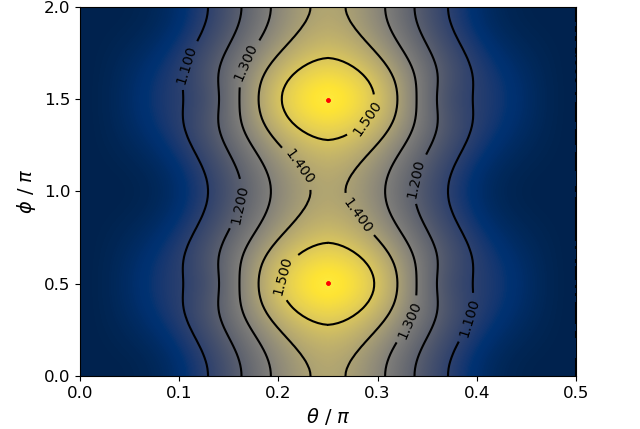
\includegraphics[scale=0.75]{2ebit_transfer.png}
    \caption{Transferring two ebits using the quantum walk protocol proposed by \cite{giordani2020}. $\theta, \phi$ are the parameters describing $\ket{\gamma}$ that defines the projection operator $\mathcal{P}_\gamma$.}
    \label{fig:2ebittransfer}
\end{figure}
*****Other coin choices gave similar results*********
Clearly whilst this proposal can be used to generate states of higher dimensional entanglement, the constraints of using quantum walk dynamics to achieve this transfer are ones that significantly hamper the efficiency of transfer.
Hence, it is worth looking at alternative models of quantum computing to adapt this protocol to in order to examine whether optimal transfer can be realised under a different set of constraints.

\section{Entanglement Transfer using Ancilla-Based Quantum Computing}
\label{section:aqc_transfer}
In this section an alternative entanglement transfer scheme is outlined.
It is designed to operate in the same setting at the QW based protocol, where there are two labs, again called $A$ and $B$, which share a common source of entangled qubits and each have their own qudits.
Analogously to the QW protocol, the qudit can be thought of as a walker driven by the ancilla qubit "coin".

The protocol can be succintly summarised by the circuit schematic given in figure \ref{fig:aqc_circuit_schematic}, and essentially is two copies of the same circuit.

\begin{figure}[h]
    \begin{center}
        \begin{tikzpicture}
            \node[scale=1.0] {
                \begin{quantikz}
                    \lstick{$\ket{0}_d^{(A)}$} & \gate{F} & \ctrl{1} & \gate{F^{-1}} & \gate{U} & \ctrl{1} & \qw\\
                    \lstick{$\ket{BS}_2^{(A)}$} & \qw & \gate{\Omega^{j}} & \qw & \qw & \gate{X} & \qw\\
                    - & - & - & - & - & - & - \\
                    \lstick{$\ket{BS}_2^{(B)}$} & \qw & \gate{\Omega^{j}} & \qw & \qw & \gate{X} & \qw\\
                    \lstick{$\ket{0}_d^{(B)}$} & \gate{F} & \ctrl{-1} & \gate{F^{-1}} & \gate{U} & \ctrl{-1} & \qw\\
                \end{quantikz}
            };
        \end{tikzpicture}
    \caption{The AQC circuit for entanglement transfer. The schematic shows two separated circuits imagined to exist in spatially separated labs, $A$ and $B$. The qudits and qubits belonging to each individual lab are labelled by their superscripts. The qubits form an entangled Bell state.}
    \label{fig:aqc_circuit_schematic}
    \end{center}
\end{figure}
The majority of the gates shown in the schematic are discussed in section \ref{subsubsection:circuits_and_gates}, with the exception of the gate $\Omega^j$.
The action of $\Omega$ in the computational basis is given by the matrix
\begin{align}
    \Omega &= 
    \begin{pmatrix}
        1 & 0\\
        0 & \omega
    \end{pmatrix}\\
    \implies \Omega^j &=
    \begin{pmatrix}
        1 & 0\\
        0 & \omega^j
    \end{pmatrix}.
\end{align}
Essentially $\Omega$ is the similar to the $Z$ operator in that it applies relative phase difference, but instead of a phase of -1, a phase corresponding to the $d^{th}$ root of unity is introduced on the $\ket{1}_2$ states, with $d$ corresponding to the dimension of the control qudits.
(Indeed, when $d=2$, $\Omega = Z$.)
Therefore the $\C{\Omega^j}$ operator is one that acts as
\begin{align}
    C\text{-}\Omega^j (\ket{x}_d\ket{y}_2) &= \ket{x}_d\otimes \Omega^{xj}\ket{y}_2\\
    & = \ket{x}_d\otimes \omega^{xyj}\ket{y}_2
\end{align}
where $\ket{x}_d$ is the control qudit and $\ket{y}_2$ the target qubit.

\begin{claim}
    \label{claim:COmegaCXinQFTbasis}
    In the Fourier basis, the $C\text{-}\Omega^j$ operator acts on the product state $\ket{+_k}_d\otimes\ket{1}_2$ to give $\ket{+_{k+j}}_d\otimes\ket{1}_2$
\end{claim}
\begin{proof}
    The Fourier basis state $\ket{+_k}_d$ is given by
    \begin{equation}
        \ket{+_k}_d = \frac{1}{\sqrt{d}}\sum_{m=0}^{d-1}\omega^{km}\ket{m}.
    \end{equation}
    Therefore
    \begin{align}
        C\text{-}\Omega^j\left(\ket{+_k}_d\ket{1}_2\right) 
        &= \frac{1}{\sqrt{d}}\sum_{m=0}^{d-1}C\text{-}\Omega^j\left(\omega^{km}\ket{m}_d\otimes\ket{1}_2\right)\\
        &= \frac{1}{\sqrt{d}}\sum_{m=0}^{d-1}\omega^{mj}\left(\omega^{km}\ket{m}_d\otimes\ket{1}_2\right)\\
        &= \frac{1}{\sqrt{d}}\sum_{m=0}^{d-1}\omega^{(k+j)m}\ket{m}_d\otimes\ket{1}_2\\
        &= \left(\frac{1}{\sqrt{d}}\sum_{m=0}^{d-1}\omega^{(k+j)m}\ket{m}_d\right)\otimes\ket{1}_2\\
        &= \ket{+_{k+j}}_d\otimes\ket{1}_2.
    \end{align}
\end{proof}
This exhibits again the counter-intuitive nature of AQC discussed in section \ref{subsection:aqc}.
Despite the qudit being the control and the qubit being the target, the only change effected is on the qudit, shifting the Fourier basis states.
Claim \ref{claim:COmegaCXinQFTbasis} also demonstrates the role of the index $j$, which essentially dictates by how many states each Fourier basis state is shifted.

The following sections demonstrate explictly how the circuit operates.

\subsection{Transfer}
\label{subsection:aqctransfer}
Assume that there are two qudits in the state $\ket{0}_d$ in labs A and B, and each lab shares a qubit each from an entangled Bell pair. The composite state is therefore given by
\begin{equation}
    \ket{00}_d^{(A,B)}\otimes\frac{1}{\sqrt{2}}\left(\ket{00}^{(A,B)}_2 + \ket{11}^{(A,B)}_2\right).
\end{equation}
Note that in the above expression, the qudits and qubits in both labs, $A$ and $B$, are in fact in the same states.
This is true for the entire running of the circuit and as such there is no need to explictly differentiate the qudits or ancilla qubits in either lab so the superscript labelling is dropped for the rest of this section.\newline

The qudits are first Fourier transformed into the Fourier basis to give
\begin{align}
    &\ket{+_0 +_0}_d\otimes\frac{1}{\sqrt{2}}\left(\ket{00}_2 + \ket{11}_2\right)\\
    &=\frac{1}{\sqrt{2}}\Big(
        \ket{+_0 +_0}_d \otimes \ket{00}_2
        +\ket{+_0 +_0}_d \otimes \ket{11}_2
        \Big).
\end{align}
The change of basis is needed because to have entanglement in the qudits, they must be in superposition of at least two states of non-zero amplitude.
Since only amplitudes can be delocalised across the qudits and ancilla qubits, in order to give other qudit states a non-zero amplitude, it is necessary to be in a basis where the basis states are related to one another by differences in their amplitudes.
The Fourier basis is one such basis where the basis states are in equal superposition of all the computational basis states but differ by the relative phases in the superposition.
Hence the need to be in the Fourier basis when using the delocalised amplitudes to effect changes in the qudit basis states.
The index $j$ on the $\Omega$ has an analogy to the QW protocol where the iteration number dictates how many steps need to be taken in the QW.
Using the same line of reasoning as outlined in Claim \ref{claim:min_steps}, on the $n^{th}$ iteration of the protocol, $j = 2^{n-1}$ so in this instance (where $n=1$) $j=1$.
Using claim \ref{claim:COmegaCXinQFTbasis}, acting $\C{\Omega}$ in both $A$ and $B$ gives the state
\begin{equation}
    \frac{1}{\sqrt{2}}\left(
        \ket{+_0 +_0}_d \otimes \ket{00}_2
        +\ket{+_1 +_1}_d \otimes \ket{11}_2
        \right).
\end{equation}
The qudits are then transformed back into the computational basis,
\begin{equation}
    \frac{1}{\sqrt{2}}\left(
        \ket{0 0}_d \otimes \ket{00}_2
        +\ket{1 1}_d \otimes \ket{11}_2
        \right).
\end{equation}
The operator $U$ is a correctional gate that essentially pairs all the even numbered computational qudit basis states with $\ket{0}_2$ and the odd numbered computational basis states with $\ket{1}_2$.
(A more complete description is given in section \ref{subsection:accumulation}.)
In this instance, $U$ can be ignored since no corrections are needed, so $\C{X}$ is directly applied, giving
\begin{align}
    &\frac{1}{\sqrt{2}}\left(
        \ket{00}_d \otimes \ket{00}_2
        +\ket{11}_d \otimes \ket{00}_2
        \right)\\
    =&\underbrace{
        \frac{1}{\sqrt{2}}\left(\ket{00}_d +\ket{11}_d\right)
    }_{\text{Bell state}}
    \otimes \ket{00}_2.    
    \label{eqn:single_aqc_transfer_final}
\end{align}
As shown in equation \ref{eqn:single_aqc_transfer_final}, the qudits now effectively form a Bell pair and the qubits are no longer entangled - the entanglement has been transferred to the qudits.

\subsection{Accumulation}
\label{subsection:accumulation}
Assume that one Bell pair has been transferred to our qudits and a second Bell pair is to be transferred.
Taking the final state given by equation \ref{eqn:single_aqc_transfer_final} and replacing the ancilla qubits with another entangled Bell pair gives
\begin{equation}
    \frac{1}{2}\left(
            \ket{00}_d +\ket{11}_d
        \right)
        \otimes 
        \left(
            \ket{00}_2 +\ket{11}_2
        \right).
\end{equation}
Again, the qudits are transformed to the Fourier basis before the $\C{\Omega^j}$ gate.
As noted in the discussion on $\C{\Omega^j}$ above, for this iteration (where $n=2$) $j=2$, giving the state
\begin{equation}
    \frac{1}{2}\Big[
            (\ket{+_0 +_0}_d + \ket{+_1 +_1}_d)\otimes\ket{00}_2
            +(\ket{+_2 +_2}_d + \ket{+_3 +_3}_d)\otimes\ket{11}_2
        \Big].
\end{equation}
After transforming back to the computational basis, the total state becomes
\begin{equation}
    \frac{1}{2}\Big[
            (\ket{00}_d + \ket{11}_d)\otimes\ket{00}_2
            +(\ket{22}_d + \ket{33}_d)\otimes\ket{11}_2
        \Big].
\end{equation}
Unlike the previous example for $n=1$, here the correctional operator $U$ is needed so that the $\C{X}$ will ensure all the qubit states are $\ket{0}_2$, allowing our qubit state to be completely separable from its associated qudit.
In order for the $\C{X}$ to do this, it must act as the identity on $\ket{0}_2$, implement an $X$ operation on $\ket{1}_2$.
Since $X$ is self inverse, the control must be in an even labelled basis state (turning $X$ into the identity) when the target is $\ket{0}_2$ and in an odd labelled basis state (leaving $X$ unchanged) when the target is $\ket{1}_2$.
Hence in this case, $U$ must implement
\begin{align}
    \ket{1} &\mapsto \ket{2}\\
    \ket{2} &\mapsto \ket{1},
\end{align}
which then gives the state
\begin{equation}
    \frac{1}{2}\Big[
            (\ket{00}_d + \ket{22}_d)\otimes\ket{00}_2
            +(\ket{11}_d + \ket{33}_d)\otimes\ket{11}_2
        \Big].
\end{equation}
As desired, $U$ has paired even numbered qudit basis states with $\ket{00}_2$ and odd numbered qudit basis states with $\ket{11}_2$.
Therefore after the $\C{X}$ operation the state becomes
\begin{align}
    &\frac{1}{2}
    (\ket{00}_d + \ket{22}_d + \ket{11}_d + \ket{33}_d)
    \otimes\ket{00}_2.
\end{align}
The two qudits are now in an entangled state with a log negativity of 2 (claim \ref{claim:maximally_entangled_states}).
This protocol can be repeated again and again with the sole change needed being the index $j$ of $\C{\Omega^j}$ and the operator $U$.
For $n>2$ there is no unique choice of $U$, as long as the end result is that even numbered states are paired with $\ket{0}_2$ and odd numbered states are paired with $\ket{1}_2$.
This can be re-expressed as requiring odd numbered states less than $\frac{d}{2}$ and even numbered states greater than or equal to $\frac{d}{2}$ to be swapped in some way.

\subsection{Retrieval}
\label{subsection:aqcretrieval}
Given that this is a circuit that solely utilises unitary transformations, retrieval of entangled Bell pairs is trivially done by running the circuit backwards. Furthermore, there is no requirement to use the same ancilla qubits to retrieve the entanglement. By the end of the circuit the ancilla qubits are in the $\ket{0}$ state, therefore any pair of ancilla qubits in the $\ket{0}$ state may be used to retrieve the entanglement.

\section{Further Uses of the AQC Circuit}
\label{section:furtheruses}
Although the goal of this research was to design a protocol in a similar setting to the QW based protocol that could optimally generate maximally entangled states, further probing of the AQC circuit shows that it has uses beyond storage of entanglement.
In this section, a scenario is considered where the quantum information contained in a collection of qubits is to be stored.
By taking one half of the circuit given for the two lab setting and adding a gate $U^{-1}$ that undoes the basis state map seen before, as shown in figure \ref{fig:aqc_qbit_store}, arbitrary qubit states can be stored in the qudit, provided that $d \geq 2^n$, where $n$ is the number of qubit states to be stored.
Furthermore, in the case that two or more qubit states are stored via this circuit then it is in fact possible to retrieve the qubit states in a different order to that in which they were stored, as long as the original order they were stored in is known.
Therefore, this circuit can be utilised in turning qudits into quantum random access memory.

\begin{figure}
    \begin{center}
        \begin{tikzpicture}
            \node[scale=1.0] {
                \begin{quantikz}
                    \lstick{$\ket{d}$} & \gate{F} & \ctrl{1} & \gate{F^{-1}} & \gate{U} & \ctrl{1} & \qw & \gate{U^{-1}} & \qw\\
                    \lstick{$\ket{b}$} & \qw & \gate{\Omega} & \qw & \qw & \gate{X} & \qw & \qw & \qw\\
                \end{quantikz}
            };
        \end{tikzpicture}
    \caption{The AQC circuit with one qudit and qubit which can store arbitrary qubit states in the qudit.}
    \label{fig:aqc_qbit_store}
    \end{center}
\end{figure}

\subsection{Quantum Random Access Memory}
\label{subsection:qram}
The procedure for utilising the circuit as a quantum random access memory is as follows.
Assume that there is a qudit in state $\ket{0}_d$ and two qubits, qubit 1 and qubit 2, in states $a\ket{0}_2 + b\ket{1}_2$ and $c\ket{0}_2 + d\ket{1}_2$ respectively.
First run the circuit with the qudit and qubit 1,
\begin{equation}\label{eqn:single_qbit_store}
    \ket{0}_d \otimes \left(a\ket{0} + b\ket{1}\right) \longrightarrow \left(a\ket{0}_d + b\ket{1}_d\right) \otimes \ket{0}_2.
\end{equation}
Then replace qubit 1 with qubit 2 and run the circuit again,
\begin{equation}
    \left(a\ket{0}_d + b\ket{1}_d\right) \otimes \left(c\ket{0}_2 + d\ket{1}_2 \right) \longrightarrow \left(ac\ket{0}_d + bc\ket{1}_d + ad\ket{2}_d + bd\ket{3}_d \right)\otimes\ket{0}_2.
    \label{eqn:twoqbitsinqdit}
\end{equation}
In order to retrieve qubit 2 back, this can be done simply by running the circuit backwards.
However, if the state of qubit 1 is to be retrieved then a specific unitary operator is first required. The form of the unitary transform can be found as follows.
Rewrite each of the qudit basis state numbers in binary, i.e.
\begin{align}
    \ket{0} &= \ket{00}\\
    \ket{1} &= \ket{01}\\
    \ket{2} &= \ket{10}\\
    \ket{3} &= \ket{11}.
\end{align}
Rewriting the final state of equation \ref{eqn:twoqbitsinqdit} in this way gives
\begin{equation}
    ac\ket{0} + bc\ket{1} + ad\ket{2} + bd\ket{3} = ac\ket{00} + bc\ket{01} + ad\ket{10} + bd\ket{11},
    \label{eqn:binaryexpression}
\end{equation}
which can be rewritten as the product state
\begin{equation}
    \underbrace{\left(c\ket{0} + d\ket{1}\right)}_{\text{Qubit 2}} \otimes \underbrace{\left(a\ket{0} + b\ket{1}\right)}_{\text{Qubit 1}}.
\end{equation}
Quite remarkably the qudit has an intuitive alternative expression as the product state of qubit 1 and qubit 2.
If the circuit is run backwards, qubit 2 will be retrieved, since it was the last qubit stored.
Therefore, to retrieve qubit 1 instead, the qudit state should be expressable as
\begin{equation}
    \underbrace{\left(a\ket{0} + b\ket{1}\right)}_{\text{Qubit 1}} \otimes \underbrace{\left(c\ket{0} + d\ket{1}\right)}_{\text{Qubit 2}}.
\end{equation}
This can be thought of as switching the positions of our two qubits, which leads us to the unitary transformation needed.
A map, $M$, is required which will switch the positions of our two qubits.
$M$ is found by mapping each of the binary qudit state representations $\{\ket{00}, \ket{01}, \ket{10}, \ket{11}\}$ to the basis state with the binary digits switched.
\begin{align}
    \ket{00} &\mapsto \ket{00}\\
    \ket{01} &\mapsto \ket{10}\\
    \ket{10} &\mapsto \ket{01}\\
    \ket{11} &\mapsto \ket{00}.
\end{align}
To verify that this does give the desired result, take the RHS of equation \ref{eqn:binaryexpression} and act $M$ on it to obtain
\begin{align}
    M\left(ac\ket{00} + ad\ket{01} + bc\ket{10} + bd\ket{11}\right) 
    &=  ac\ket{00} + ad\ket{10} + bc\ket{01} + bd\ket{11}\\
    &= \underbrace{\left(a\ket{0} + b\ket{1}\right)}_{\text{Qubit 1}} \otimes \underbrace{\left(c\ket{0} + d\ket{1}\right)}_{\text{Qubit 2}},
\end{align}
as required.
$M$ can be expressed in terms of the original qudit state labelling by converting the binary back
\begin{align}
    \ket{0} &\mapsto \ket{0}\\
    \ket{1} &\mapsto \ket{2}\\
    \ket{2} &\mapsto \ket{1}\\
    \ket{3} &\mapsto \ket{3}.
\end{align}
The matrix representation of $M$ is given by
\begin{equation}
    M = 
    \begin{pmatrix}
        1 & 0 & 0 & 0\\
        0 & 0 & 1 & 0\\
        0 & 1 & 0 & 0\\
        0 & 0 & 0 & 1\\
    \end{pmatrix}.
\end{equation}
Generalising this to larger numbers of qubits stored is done via the same thought process.
Imagine that there is now third qubit to be stored in the qudit, qubit 3, in the state
\begin{equation}
    e\ket{0} + f\ket{1}.
\end{equation}
When qubits 1, 2 and 3 are stored in that same order, it results in the state
\begin{equation}
    ace\ket{0} + ade\ket{1} + bce\ket{2} + bde\ket{3} + ace\ket{4} + adf\ket{5} + bcf\ket{6} + bdf\ket{7},
\end{equation}
which again, when converted to binary numbers, can be expressed as the product state
\begin{equation}
    \underbrace{\left(e\ket{0} + f\ket{1}\right)}_{\text{Qubit 3}} \otimes \left(c\ket{0} + d\ket{1}\right) \otimes \underbrace{\left(a\ket{0} + b\ket{1}\right)}_{\text{Qubit 1}}.
\end{equation}
If the state of qubit 1 is needed, then $M$ must switch the first and last qubits, and therefore must implement the map
\begin{align}
    \ket{1} = \ket{001} &\mapsto \ket{100} = \ket{4}\\
    \ket{3} = \ket{011} &\mapsto \ket{110} = \ket{6}\\
    \ket{4} = \ket{100} &\mapsto \ket{001} = \ket{1}\\
    \ket{6} = \ket{110} &\mapsto \ket{011} = \ket{3}
\end{align}
with all other basis states mapped to themselves as they are identical when switching the first and last digits of their binary representations.
Having operated $M$ on the qudit state, the circuit can be run backwards in order to retrieve qubit 1. As with retrieving Bell pairs in section \ref{section:aqc_transfer}, any qubit in the state $\ket{0}$ can be used to retrieve qubit 1. A proof that this circuit can store any number of qubit states is given in appendix \ref{appendix:any_num_qubits}.

In a practical setting it may be more efficient to build a gate, $P$, that permutes the order of the qubits instead of swapping two digits.
One example of $P$ would be the map that permutes each qubit one place the right,
\begin{align}
    \ket{1} = \ket{001} &\mapsto \ket{100} = \ket{4}\\
    \ket{2} = \ket{010} &\mapsto \ket{001} = \ket{1}\\
    \ket{3} = \ket{011} &\mapsto \ket{101} = \ket{5}\\
    \ket{4} = \ket{100} &\mapsto \ket{010} = \ket{2}\\
    \ket{5} = \ket{101} &\mapsto \ket{110} = \ket{6}\\
    \ket{6} = \ket{110} &\mapsto \ket{011} = \ket{3}.
\end{align}
Again $\ket{0}, \ket{7}$ are mapped to themselves as the permutation does not affect them.
In this way, any of the qubit states can be retrieved by continually applying $P$ until the qubit state to be retrieved is in the right "place".
Utilising a single gate would also be more appropriate for the ancilla-based quantum computing setting where a minimal gate set is desired for the control qudits.
However, this would require multiple applications of the same gate which, without adequate error correction, would lead to greater decoherence of the quantum information than if just a single swapping gate $M$ were applied.

\section{Discussion}
\label{section:discussion}
In the example given in section \ref{section:qw_transfer}, it is shown that the protocol proposed in the QW setting can optimally transfer all the entanglement to the qudit pair.
However, this is with the significant caveat that the example does not use quantum walk dynamics in order to transfer the entanglement, as using the identity as a coin is akin to having no coin at all.
In analysing the protocol with the Hadamard coin, it was only possible to transfer one Bell state's worth of entanglement optimally and
numerical simulations of the protocol for storing two Bell states, found that the resulting state had around 1.585 units of log negativity (figure \ref{fig:2ebittransfer}).
Furthermore, the projective measurements employed as part of the protocol mean that it is not a unitary protocol, therefore not deterministic and non-trivial to reverse in order to retrieve the entanglement out from the entangled qudits.
The experimental implementation suggested in the paper also required the use of post selection, where undesirable states were discarded and the protocol run again.
All this in combination results in a protocol which is rather inefficient in achieving its aims, and serves more as a proof of concept in that it is possible to use quantum walk dynamics to transfer entanglement, but falls short in being a suitable implementation for the task.

Adapting the identity coin example to the ancilla-based quantum computing circuit given in section \ref{section:aqc_transfer} resulted in a circuit that solved these inefficiencies.
The entanglement can always be transferred optimally and exclusive utilisation of unitary operators means that the circuit can just be reversed with any ancilla qubit in the $\ket{0}$ state.

\subsection{Further Steps}
\label{subsection:furthersteps}
As discussed in Section \ref{section:furtheruses}, the circuit given in figure \ref{fig:aqc_circuit_schematic} has potential uses beyond the original scope in which is has been designed.
It would be of interest to see if it can also be applied to transferring multipartite entanglement to higher dimensions, for example the entanglement in transferring GHZ states or W states.
Further analysis to see if Bell states could be used to generate multipartite entangled states would also be interesting to carry out.
The analysis of this work could be brought to greater completion if the circuit was generalised to transferring entanglement between qudit pairs of arbitrary dimension instead of just entangled Bell pairs, although this would likely be more for academic rather than practical purposes, since the practical goal of the circuit is to take advantage of Bell pair generating schemes to generate higher dimensional entanglement.

\subsection{Conclusions}
\label{subsection:conclusions}
Overall, the QW protocol aims to solve an interesting problem with a suitable set of contraints that might be realistic ones to consider in future as quantum computing technologies develop.
In principle it does away with the need to repeatedly design different entanglement schemes for qudits of differing dimension, since the same scheme can used to accumulate entanglement in any dimension, just by using entangled Bell states to transfer the entanglement from.
However, it was shown that in practice this protocol scaled inefficiently as more entanglement was transferred when actually using quantum walk dynamics, and optimal transfer is not possible..
It also suffers from difficulties in transferring entanglement back to the qubits due to its non-unitary nature.
Post-selection is also needed further decreasing the efficiency of the protocol.\newline

Instead, an alternative scheme was proposed to operate in the same physical setting, but based on an AQC model which came with a slightly different set of constraints.
It was shown that this alternative scheme is able to achieve optimal transfer of entanglement, no matter the number of Bell states to be stored.
Retrieval of entangled Bell pairs is also simple to do, since the entirety of the protocol was unitary, and retrieval amounted to reversing the circuit given in figure \ref{fig:aqc_circuit_schematic}.
Furthermore, it was also shown that the circuit had further uses outside of entanglement transfer and could be utilised to turn qudits into quantum random access memory.
This increased versatility gives greater practical benefits to the AQC circuit as only one circuit is needed to achieve multiple aims.
Its relative simplicity also makes it an effective circuit to implement on a practical quantum computer, with only a select few gates needed to implement it.

\begin{acknowledgements}
    \addcontentsline{toc}{section}{Acknowledgements}
    I would like to thank Dr Viv Kendon for her insight and advice during this research, especially during the challenging conditions we found ourselves having to work in.
\end{acknowledgements}

\printbibliography[heading=bibintoc]

\newpage

\appendix
\appendixpage
\addappheadtotoc
\setcounter{equation}{0}
\renewcommand{\theequation}{A.\arabic{equation}}
\section{Proof that the circuit can store any number of qubits}
Here it is proven by induction that the circuit presented in section \ref{section:furtheruses} can store $n\in\mathbb{N}$ qubit states into the qudit, as long as the dimension of the Hilbert space $d\geq 2^n$.
\begin{proof}$ $\newline
    $n=1$\newline
    It has already been shown in equation \ref{eqn:single_qbit_store} that a single arbitary qubit state can be stored giving
    \begin{equation}
        (a_1\ket{0}_d + b_1\ket{1}_d)\otimes\ket{0}_2,
    \end{equation}
    where the coefficients have been relabelled $a \rightarrow a_1, b\rightarrow b_1$.
    \newline

    $n = k$\newline
    Assume that $n$ qubit states have been stored in the qudit, giving the qudit state
    \begin{equation}
        \left(\sum_{j=0}^{2^k - 1}c_j\ket{j}_d\right)\otimes\ket{0}_2.
        \label{eqn:sum_qudit_state}
    \end{equation}
    Furthermore, assume that this can be re-expressed as a tensor product of $n$ qubits by converting the computational basis state labels to their binary equivalents and "expanding" to give
    \begin{align}
        (a_k\ket{0} + b_k\ket{1})\otimes(a_{k-1}\ket{0} + b_{k-1}\ket{1})\otimes\cdots\otimes(a_1\ket{0} + b_1\ket{1})\otimes\ket{0}_2\\
        =&\bigotimes_{i = k}^{1}\left(a_i\ket{0} + b_i\ket{1}\right)\otimes\ket{0}_2,
    \end{align}
    where the coefficients $a_{i}$ and $b_{i}$ match the amplitudes of the $i^{th}$ qubit state that was stored.
    Note that the assumption that the state can be expanded in such a way implies equation \ref{eqn:sum_qudit_state} where
    \begin{equation}
        c_j = \prod_{i=1}^{k}(a_i \delta^{0}_{j_{2_i}} + b_i\delta^{1}_{j_{2_i}}),
    \end{equation}
    where $j_{2_i}$ is the $i^{th}$ digit of the binary expression of $j$, and $\delta$ is the Kronecker delta.\newline

    $n=k+1$\newline
    The entire state prior to running the circuit with an additional qubit to be stored is given by
    \begin{align}
        &\left(\bigotimes_{i = k}^{1}(a_i\ket{0} + b_i\ket{1})\right)\otimes(a_{k+1}\ket{0}_2 + b_{k+1}\ket{1}_2)\\
        =&\left(\bigotimes_{i = k}^{1}(a_i\ket{0} + b_i\ket{1})\right)\otimes a_{k+1}\ket{0}_2\label{eqn:first_summand}\\ 
        +
        &\left(\bigotimes_{i = k}^{1}(a_i\ket{0} + b_i\ket{1})\right)\otimes b_{k+1}\ket{1}_2. \label{eqn:second_summand}
    \end{align}
    This state is now put through the circuit.
    Note that the summand which is tensored with $\ket{0}_2$ is not affected by the $\C{\Omega^j}$ since the target is $\ket{0}_2$.
    Therefore only the summand tensored with $\ket{1}_2$ is advanced, and by claim \ref{claim:COmegaCXinQFTbasis}, the basis states are shifted up by $j$ steps.
    From claim \ref{claim:min_steps}, for the $\C{\Omega^j}$ gate, $j = 2^k$.
    Consider what this means in terms of computational basis states.
    When written terms of computational basis states, \crefrange{eqn:first_summand}{eqn:second_summand} are given by the sum
    \begin{align}
        &\left(\sum_{i=0}^{2^k - 1}c_i\ket{i}_d\right) \otimes a_{k+1}\ket{0}_2\\
        +&\left(\sum_{i=0}^{2^k - 1}c_i\ket{i}_d\right) \otimes b_{k+1}\ket{1}_2.
    \end{align}
    Shifting all of the computational basis states in the second summand by $j=2^k$ yields
    \begin{align}
        &\left(\sum_{i=0}^{2^k - 1}c_i\ket{i}_d\right) \otimes a_{k+1}\ket{0}_2\\
        +&\left(\sum_{i=0}^{2^k - 1}c_i\ket{i + 2^k}_d\right) \otimes b_{k+1}\ket{1}_2.
    \end{align}
    In binary, adding $2^k$ to a number that is less than $2^k$ can be thought of as placing an additional 1 at the start of the string of binary digits.
    For example, where $(x)_2$ denotes that the number $x$ is written in binary,
    \begin{equation}
        7 + 8 = (2^3 - 1) + (2^3) = (111)_2 + (1000)_2 = (1111)_2.
    \end{equation}
    In this way, the action of the $\C{\Omega^j}$ gate on the tensor representation of the qudit given in \crefrange{eqn:first_summand}{eqn:second_summand} can be thought of as adding a $\ket{1}$ in front of all of the binary representations of the computational basis states tensored with $\ket{1}_2$.
    Similarly, a $\ket{0}$ can be added in front of the binary representations of the computational basis states tensored with $\ket{0}_2$, since it still represents the same number ($01 = 1$).
    \begin{align}
        &\ket{0} \otimes \left(\bigotimes_{i = k}^{1}(a_i\ket{0} + b_i\ket{1})\right)\otimes a_{k+1}\ket{0}_2\\ 
        +
        &\ket{1} \otimes \left(\bigotimes_{i = k}^{1}(a_i\ket{0} + b_i\ket{1})\right)\otimes b_{k+1}\ket{1}_2\\
        =  &a_{k+1}\ket{0} \otimes \left(\bigotimes_{i = k}^{1}(a_i\ket{0} + b_i\ket{1})\right)\otimes \ket{0}_2\\ 
        +
        &b_{k+1} \ket{1} \otimes \left(\bigotimes_{i = k}^{1}(a_i\ket{0} + b_i\ket{1})\right)\otimes \ket{1}_2.
    \end{align}
    It is only possible to add these additional kets if the $d \geq 2^{k+1}$, else the Hilbert space is not large enough to accomodate the additional states being represented, hence the need for that contraint.
    The next step of the circuit is to use some map $U$ to pair the even numbered computational basis states with $\ket{0}_2$ and the odd numbered computational basis states with $\ket{1}_2$ to convert the $\ket{1}_2$ to a $\ket{0}_2$ via a $\C{X}$ operation, after which $U$ is uncomputed.
    On the qudit state, since no amplitude changes are involved this is akin to doing a $UU^{-1}=I$ and so leaves the qudit state untouched.
    Therefore the final state is given by
    \begin{align}
        &a_{k+1}\ket{0} \otimes \left(\bigotimes_{i = k}^{1}(a_i\ket{0} + b_i\ket{1})\right)\otimes \ket{0}_2\\ 
        +
        &b_{k+1} \ket{1} \otimes \left(\bigotimes_{i = k}^{1}(a_i\ket{0} + b_i\ket{1})\right)\otimes \ket{0}_2\\
        =&\left(a_{k+1}\ket{0}+b_{k+1} \ket{1}\right) \otimes \left(\bigotimes_{i = k}^{1}(a_i\ket{0} + b_i\ket{1})\right)\otimes \ket{0}_2\\
        =&\left(\bigotimes_{i = k+1}^{1}(a_i\ket{0} + b_i\ket{1})\right)\otimes \ket{0}_2
    \end{align}
    So the statement is true by induction.
\end{proof}

\end{document}